Im neuen Projektablauf des Lösungsansatz wurde an diversen Stellen auf Instrumente
verwiesen, für die in diesem Kapitel noch die richtige Wahl getroffen werden
muss. Als erstes werden die einzelnen Verwendungen aufgelistet und beschrieben.
In einem weiteren Schritt werden verschiedene Varianten verglichen. Danach
kann die Geschäftsleitung der allink entscheiden, welche Instrumente sie
in Zukunft einsetzen möchte.

\subsection{Anforderungen aus dem Projektablauf}
In der nachfolgenden Tabelle \ref{tab:projektablauf_instrumente} sind alle
Anforderungen an Instrumente, auf die im Projektablauf verwiesen wurde, aufgelistet 
und beschrieben.

\begin{longtable}{lp{14cm}}
    \toprule \textbf{Nr.} & \textbf{Beschreibung} \\
    \midrule AI1 & Ein Instrument, um ein neues Projekt zu eröffnen und um eine 
        eindeutige Projektnummer zu vergeben. \\
    \midrule AI2 & Ein Instrument, mit dem alle Projektmitarbeiter ihre 
        aufgewendeten Stunden rapportieren können. \\
    \midrule AI3 & Ein Instrument, um die Arbeitspakete bzw. Todos eines Projektes
        verwalten und überwachen zu können. \\
    \midrule AI4 & Ein Instrument, um die Ressourcenplanung erstellen zu können. \\
    \midrule AI5 & Ein Instrument, um die Meilensteine eines Projektes verwalten 
        und überwachen zu können.\\
    \midrule AI6 & Ein Instrument, um die Geldflüsse wie Offerten, Rechnungen 
        und Teilzahlungen verwalten und überwachen zu können. \\
    \midrule AI7 & Ein Instrument und Vorgaben, um alle Projektdaten archivieren 
        zu können. \\
    \bottomrule
    \caption[Im Projektablauf benötigte Instrumente]{Im Projektablauf benötigte 
        Instrumente\footnotemark}
    \label{tab:projektablauf_instrumente}
\end{longtable}
\footnotetext{Eigene Darstellung}

Es können natürlich mehrere Instrumente mit einer Variante abgedeckt werden.
Zum Beispiel mit der Projektmanagementsoftware Metronom\footnote{Metronom ist die 
Projektmanagementsoftware welche die FEINHEIT GmbH einsetzt.
Vgl. Kapitel \ref{chap:branchenvergleich}.}. Sie wurden jedoch absichtlich getrennt 
aufgelistet, damit für jedes Instrument verschieden Varianten aufgezeigt werden können.

\subsection{Instrumentenvergleich}
\newcounter{vcounter}
In der nachfolgenden Tabelle \ref{tab:instrumenten_varianten} sind alle
Instrumente, und somit alle möglichen Varianten die zur Auswahl stehen, aufgelistet 
und beschrieben. Die zur Auswahl stehenden Instrumente wurden zusammen mit der
Geschäftsleitung evaluiert.

Natürlich gibt es diverse weitere Produkte um diese
Anforderungen abdecken zu können. Diese wurden aber zusammen mit der Geschäftsleitung
der allink beschränkt, da zum Beispiel eine SAP-Lösung\footnote{SAP bietet angepasste
Softwarelösungen für sämtliche Geschäftsprozesse eines Unternehmens.} gar 
nicht in Frage kommen würde und somit nicht weiter betrachtet werden muss.
Auch fällt eine vollständige Eigenentwicklung weg, da allink sich in Zukunft nicht
um die Pflege eines ganzen Projektmanagement Systems kümmern möchte. Erweiterungen
bestehender Systeme werden aber in Betracht gezogen, sofern die Systeme dies
ermöglichen.

Im Fokus stehen nun noch die Projektmanagement Software Metronom und Basecamp\footnote{Basecamp
ist eine webbasierte Projektmanagement Software von 37signals, \url{http://basecamphq.com/}}.
Die API\footnote{Eine API ist eine Programmierschnittstelle, die ein System zur Verfügung 
stellt um anderen Systemen die darin verwalteten Informationen zugänglich zu machen.} 
von Basecamp zur Anbindung weiterer Software ist zudem für eigene Erweiterungen 
sehr interessant.

\begin{longtable}{lllp{8cm}}
    \toprule
    \textbf{Anf.} & \textbf{Nr.} & \textbf{Instrument} & \textbf{Beschreibung} \\
    
    \midrule AI1 
    & \addtocounter{vcounter}{1}I\arabic{vcounter} & Metronom & Die webbasierte 
        Projektmanagement Software Metronom bietet eine Projektverwaltung an. \\
    & \addtocounter{vcounter}{1}I\arabic{vcounter} & Basecamp & Die ebenfalls 
        webbasierte Projektmanagement Software Basecamp
        bietet auch eine Projektverwaltung an. \\
    
    \midrule AI2 
    & \addtocounter{vcounter}{1}I\arabic{vcounter} & Metronom & Metronom bietet 
        die Möglichkeit Zeit auf sogenannte Tickets zu rapportieren. \\
    & \addtocounter{vcounter}{1}I\arabic{vcounter} & Basecamp & Basecamp bietet
        ebenfalls die Möglichkeit Zeit auf ein Projekt oder Todo zu rapportieren. \\
    & \addtocounter{vcounter}{1}I\arabic{vcounter} & Basecamp Erweiterung & Dank
        der API von Basecamp könnte eine kleine Software entwickelt werden, die
        das Rapportieren dem Mitarbeiter so einfach wie möglich macht, jedoch
        die Daten weiterhin im Basecamp ablegt. \\
    
    \midrule AI3
    & \addtocounter{vcounter}{1}I\arabic{vcounter} & Metronom & Mit Metronom können
        die laufenden Arbeitspakete und Tickets eines Projektes verwaltet und
        überwacht werden. \\
    & \addtocounter{vcounter}{1}I\arabic{vcounter} & Basecamp & Basecamp bietet
        ebenfalls das Verwalten und Überwachen von Arbeitspaketen und Todos an. \\
    
    \midrule AI4 
    & \addtocounter{vcounter}{1}I\arabic{vcounter} & Metronom & Metronom ermöglicht
        nur eine beschränkte Ressourcenplanung. Man kann die Summe aller geplanten
        Tickets pro Mitarbeiter auswerten. \\
    & \addtocounter{vcounter}{1}I\arabic{vcounter} & Excel & Die Ressourcenplanung
        könnte auch in einem Microsoft Excel oder Apple Numbers File geführt werden. \\
    & \addtocounter{vcounter}{1}I\arabic{vcounter} & Eigenentwicklung & Für die
        Ressourcenplanung könnte allink eine eigene Software mit Fokus auf
        ihre Bedürfnisse entwickeln und ebenfalls an z.B. Basecamp koppeln. \\
    
    \midrule AI5 
    & \addtocounter{vcounter}{1}I\arabic{vcounter} & Metronom & Mit Metronom
        können Meilensteine geplant und verwaltet werden. \\
    & \addtocounter{vcounter}{1}I\arabic{vcounter} & Basecamp & Auch Basecamp
        bietet die Möglichkeit Meilensteine zu planen und zu verwalten.\\
    
    \midrule AI6 
    & \addtocounter{vcounter}{1}I\arabic{vcounter} & Metronom & Metronom bietet
        auch hier alle nötigen Funktionen um die Geldflüsse zu planen. Jedoch
        ist die Software bei der Darstellung von den Übersichten und Rechnungen
        sehr eingeschränkt. \\
    & \addtocounter{vcounter}{1}I\arabic{vcounter} & Eigenentwicklung & Hier
        könnte allink ebenfalls eine eigene Software mit Anbindung an
        Basecamp entwickeln, um genau ihre Bedürfnisse abdecken zu können.\\
    
    \midrule AI7 
    & \addtocounter{vcounter}{1}I\arabic{vcounter} & allink Server & Hier kann
        der schon vorhandene Fileserver von allink eingesetzt werden.\\
    
    \bottomrule
    \caption[Zur Auswahl stehende Varianten der Instrumente]{Zur Auswahl stehende 
        Varianten der Instrumente\footnotemark}
    \label{tab:instrumenten_varianten}
\end{longtable}
\footnotetext{Eigene Darstellung}

\subsection{Variantenentscheid}
Obwohl Metronom bei der Auflistung der Varianten öfters gewählt werden könnte,
hinterlässt die Software beim Testen einen eher schwerfälligen Eindruck.
Basecamp wurde von allink schon öfters in Projekten mit anderen Agenturen 
verwendet und hat bis jetzt nur Anklang gefunden.

Nach längeren Diskussionen mit der Geschäftsleitung entscheidet sich die allink
für die Projektmanagement Software Basecamp und die Umsetzung von eigenen Erweiterungen. So muss
sich allink nicht um den Kern der Software kümmern und kann für ihre Bedürfnisse
passende Erweiterungen entwickeln. Somit wurde entschieden die Instrumente I2,
I5, I7, I10, I12, I14 und I15 einzusetzen. In der nachfolgenden Abbildung \ref{pic:04_systemlandschaft} 
ist die neu geplante Systemlandschaft des Projektmanagements skizziert.

\begin{figure}[htbp]
\begin{center}
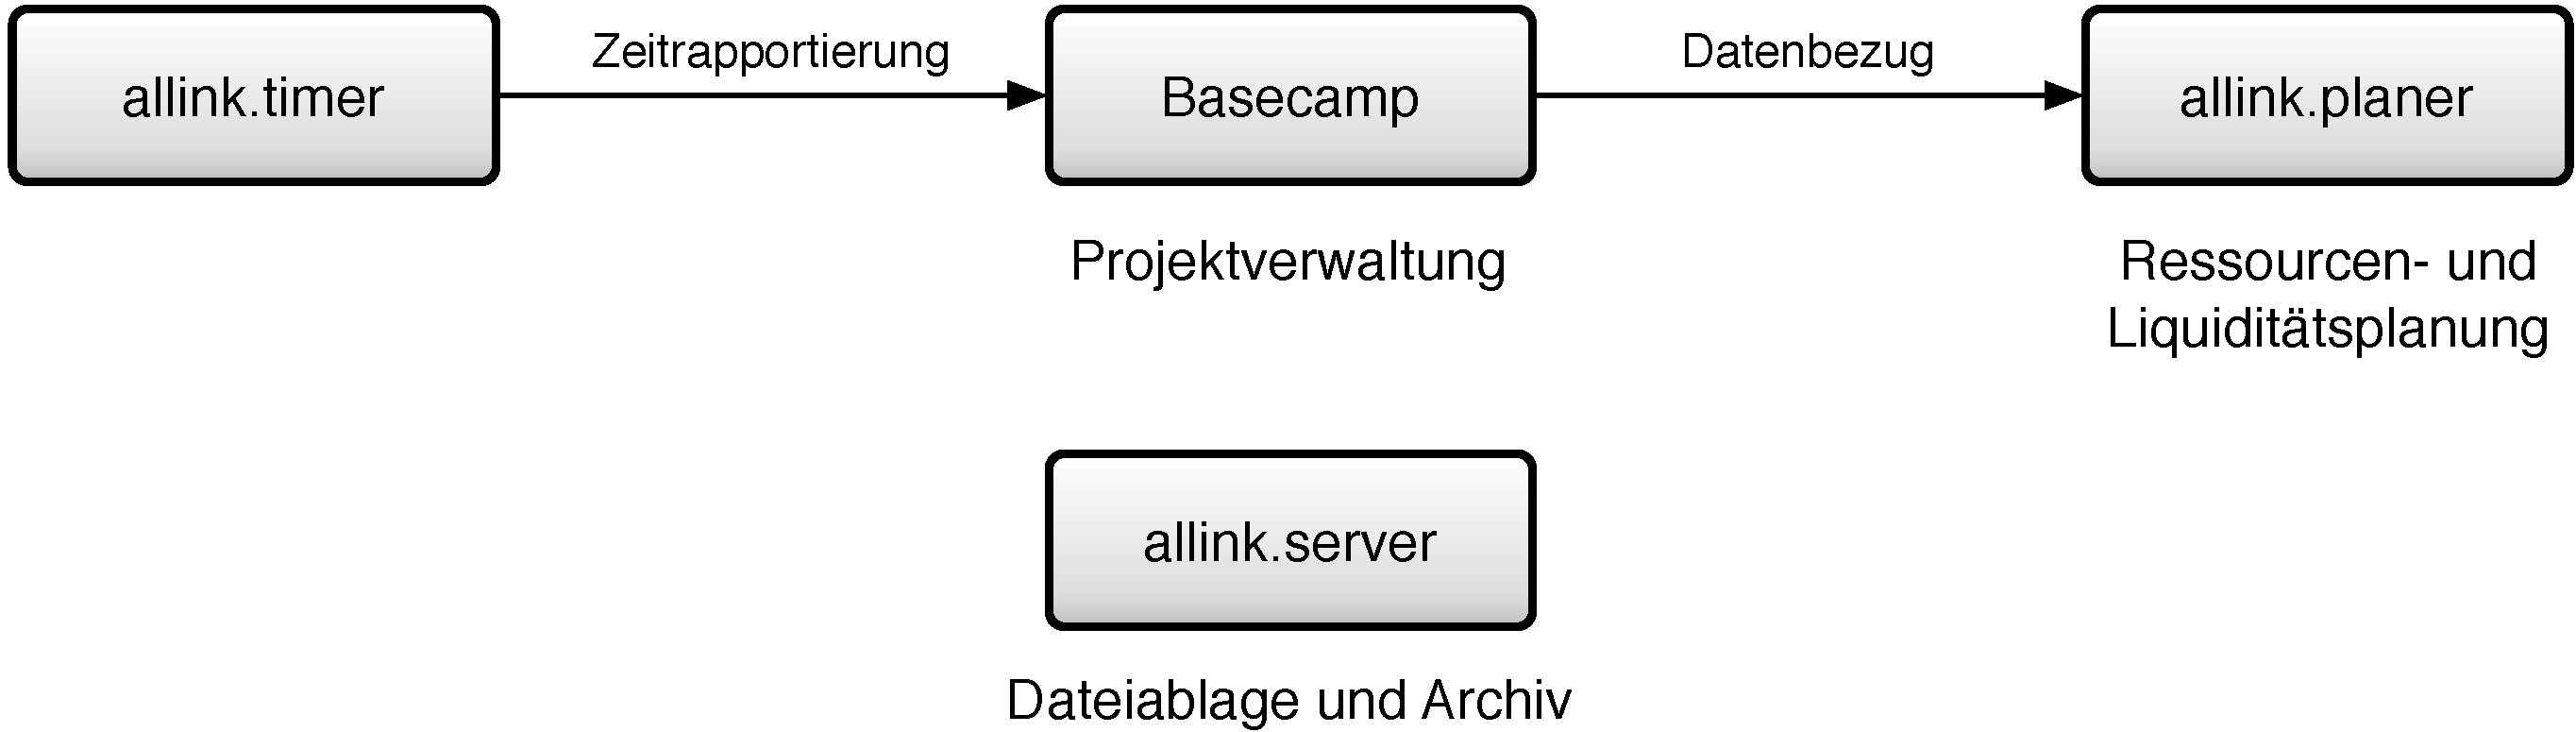
\includegraphics[width=0.8\textwidth,angle=0]{./bilder/loesung/04_systemlandschaft.pdf}
\caption[Neu geplante Systemlandschaft des Projektmanagements]{Neu geplante 
    Systemlandschaft des Projektmanagements\footnotemark}
\label{pic:04_systemlandschaft}
\end{center}
\end{figure}
\footnotetext{Eigene Darstellung}

Nachfolgend wird auf die einzelnen Elemente der neuen Systemlandschaft
eingegangen und jeweils auf die erfüllende Anforderung aus dem neuen Projektablauf
verwiesen.

\subsubsection{Basecamp}
Als zentrales Element dient neu die kostenpflichtige Projektmanagement Software 
Basecamp zur Erfassung und Verwaltung der Projekte (\textbf{AI1}). Darin werden alle
Arbeitspakete, Todos, Meilensteine und die rapportierten Stunden geführt (\textbf{AI3} 
und \textbf{AI5}). Basecamp bietet, wie bereits erwähnt, eine Schnittstelle um
andere Systeme anzubinden. Diese wird in den zwei nachfolgenden Eigenentwicklungen
genutzt.

\subsubsection{allink.timer}
Es wird eine kleine Software namens allink.timer entwickelt, worüber Mitarbeiter 
möglichst einfach ihre Stunden pro Projekt rapportieren können (\textbf{AI2}). 
Diese Software bezieht die laufenden Projekte aus Basecamp und speichert die 
rapportierten Stunden wieder zurück.

\subsubsection{allink.planer}
Für die Ressourcenplanung und die Planung der Geldfüsse wird zusätzlich eine 
Software names allink.planer entwickelt. Darin werden alle Ressourcen, Offerten, 
Rechnungen und Teilzahlungen verwaltet und überwacht (\textbf{AI4} und \textbf{AI6}).
Es wurde bereits jetzt über eine zukünftige Erweiterung diskutiert, um 
Offerten und Rechnungen direkt aus dieser Software generieren zu können.

\subsubsection{allink.server}
Für die Ablage und Archivierung der Projektdaten wird der schon vorhanden
allink Server verwendet (\textbf{AI7}). Alle Mitarbeiter werden Zugriff auf die Unterlagen
von laufenden wie auch archivierte Projekten haben. Die Projektstruktur
wurde zusammen mit der Geschäftsleitung definiert und soll für laufende
wie auch archivierte Projekte, wie in der folgenden Abbildung \ref{pic:05_ablagestruktur} 
dargestellt, aufgebaut sein.

\begin{figure}[htbp]
\begin{center}
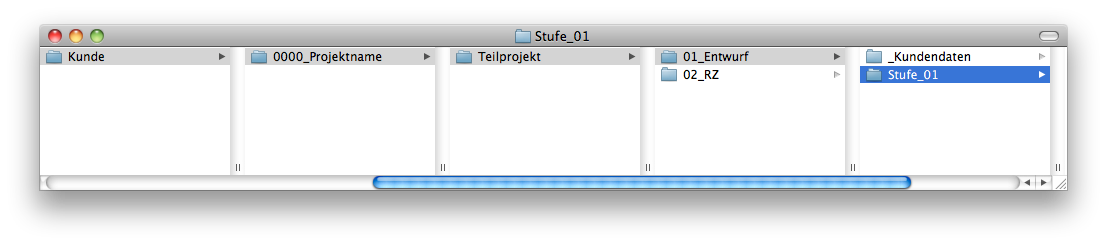
\includegraphics[width=1.0\textwidth,angle=0]{./bilder/loesung/05_ablagestruktur.png}
\caption[Ablagestruktur laufender und archivierter Projekte]{Ablagestruktur 
    laufender und archivierter Projekte\footnotemark}
\label{pic:05_ablagestruktur}
\end{center}
\end{figure}
\footnotetext{Eigene Darstellung}

Pro Kunde existiert ein, mit dem Namen des Kunden beschrifteter, Ordner. Darin befindet
sich pro Projekt jeweils ein Ordner mit genauer Projektbezeichnung inklusive Projektnummer.
Darin kann, sofern notwendig, noch in Teilprojekte unterschieden und
pro Teilprojekt ein Ordner erstellt werden. Im Projekt- oder Teilprojektordner
existieren im Minimum ein Ordner ``01 Entwurf'' und ``02 RZ'', wobei RZ für Reinzeichnung
steht. Im Reinzeichnungsordner werden die am Ende verwendeten Dateien abgelegt.
In den Entwurfsordner werden Kundendaten und die verschiedenen Stufen der Entwürfe
abgelegt.

\subsection{Überblick der Softwareveränderung}
Durch den Entscheid, welche Software in Zukunft im Projektmanagement eingesetzt
wird, verändert sich die Softwarelandschaft bei allink. In der nachfolgenden
Tabelle \ref{tab:neu_verwendete_software} wird alle Software aufgelistet, die 
bisher eingesetzt wurde\footnote{Vgl. Kapitel \ref{chap:verwendete_software}} 
und neu eingekauft oder entwickelt wird.

\newcounter{scounter}
\begin{longtable}{lllll}
    \toprule \textbf{Nr.} & \textbf{Bezeichnung} & \textbf{Hersteller} & \textbf{Kategorie} & \textbf{Status} \\
    \midrule \addtocounter{scounter}{1}S\arabic{scounter} & MacOS X & Apple & 
        Betriebssystem & wird beibehalten \\
    \midrule \addtocounter{scounter}{1}S\arabic{scounter} & Microsoft Windows & 
        Microsof & Betriebssystem & wird beibehalten \\
    \midrule \addtocounter{scounter}{1}S\arabic{scounter} & MacOS X Server & Apple & 
        Betriebssystem & wird beibehalten \\
    \midrule \addtocounter{scounter}{1}S\arabic{scounter} & Apple iWork & Apple & 
        Office Suite & wird beibehalten \\
    \midrule \addtocounter{scounter}{1}S\arabic{scounter} & Microsoft Office & 
        Microsoft & Office Suite & wird beibehalten \\
    \midrule \addtocounter{scounter}{1}S\arabic{scounter} & Apple Mail & Apple & 
        E-Mail Software & wird beibehalten \\
    \midrule \addtocounter{scounter}{1}S\arabic{scounter} & Stundenwidget & allink & 
        Dashboardwidget & wird abgelöst \\
    \midrule \addtocounter{scounter}{1}S\arabic{scounter} & Basecamp & 37signals & 
        Projektmanagement & wird eingekauft \\
    \midrule \addtocounter{scounter}{1}S\arabic{scounter} & allink.timer & allink & 
        Projektmanagement & wird entwickelt \\
    \midrule \addtocounter{scounter}{1}S\arabic{scounter} & allink.planer & allink & 
        Projektmanagement & wird entwickelt \\
    \bottomrule
    \caption[Neue Softwarelandschaft bei allink]{Neue Softwarelandschaft bei allink\footnotemark}
    \label{tab:neu_verwendete_software}
\end{longtable}
\footnotetext{Eigene Darstellung}

Die Software Basecamp wurde nach der Entscheidung von allink eingekauft.
Mit der Entwicklung der Projektmanagement Tools allink.timer und allink.planer
wurde bereits begonnen. Der Studierende hat zwei funktionierende Prototypen 
erstellt. Da die Softwareentwicklung nicht Bestandteil dieser Arbeit ist, wird
auf eine ausführliche Dokumentation verzichtet. Sie werden jedoch im ``Proof of
Concept'' im Kapitel \ref{chap:proof_of_concept} zur Anwendung kommen.
